\chapter{Project Idea}
\section{Problem Domain}
We defined in our opinion the most important domains which a Reverse Engineer has to have knowledge of.
\begin{figure}[H]
    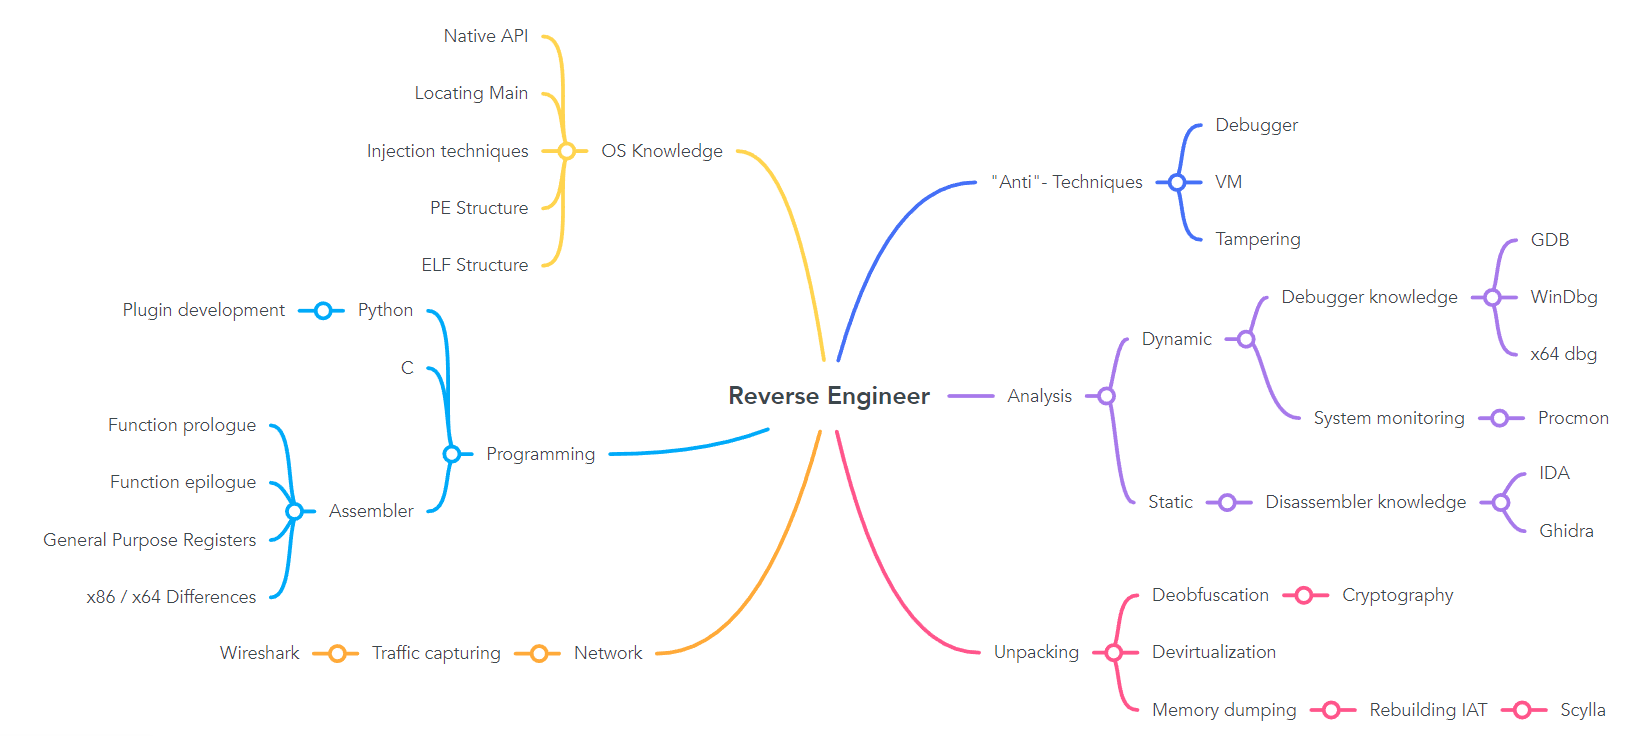
\includegraphics[width=\linewidth, center]{resources/ReverseEngineeringDomain.png}
    \caption{Mindmap of the knowledge a Reverse Engineer needs.}
    \label{fig:mindmap}
\end{figure}

\section{Learning Concepts}
Based on the Problem Domain from the last section we decided the most basic domains were programming, analysis and OS knowledge. So we decided that we are going to create the most labs and the first ones about these topics and then the later introduce the other domains in later Labs. We want to focus on Linux and Windows.

\noindent We also decided that we can expect for Students to already know about C, Python and some basic knowledge about Assembler because everyone has to have had BSYS which teaches about Assembler and C. Automation with python is also a module which now is in every sample curriculum at the OST.

\begin{center}
    \begin{table}[H]
        \centering
        \begin{tabular}{ |p{4.1cm}|p{10cm}| } 
            \hline
                Topic & 
                Description \\ [0.5ex] 
            \hline
            \hline
                Refresher & 
                Give the students some little refreshing on the key topics (Assembly)  \\ 
            \hline
                Introduction to RE \#1 & 
                Explain analysis approaches (Dynamic / Static) and install tools \\ 
            \hline
                Introduction to RE \#2 & 
                Given a simple C file, students compile it and try to find a key (Static) (Find Main function) \\ 
            \hline
                Introduction to RE \#3 & 
                Given a simple C file, students compile it and try to find a key (Dynamic) (learn GDB / x64) \\ 
            \hline
                First RE attempts & 
                Given simple files compiled in several languages (PY, C\#, C++) get flag \\ 
            \hline
                First keygen & 
                Not only finding out the password but writing a keygen for the program \\
            \hline
                Harder CrackMes & 
                Introduce new native API funcs / techniques like stack strings \\
            \hline
                Injection techniques & 
                Explain some injection techniques \\
            \hline
                Dump memory & 
                Explain how to dump memory off a given executable which uses a previously explained injection technique \\
            \hline
                "Anti"-Techniques & 
                Introduce "Anti"-Techniques and provide program for students to bypass \\
            \hline
        \end{tabular}
        \caption{Overview of all the Labs.}
    \end{table}
\end{center}